% Customizable fields and text areas start with % >> below.
% Lines starting with the comment character (%) are normally removed before release outside the collaboration, but not those comments ending lines

% svn info. These are modified by svn at checkout time.
% The last version of these macros found before the maketitle will be the one on the front page,
% so only the main file is tracked.
% Do not edit by hand!
\RCS$Revision: 248927 $
\RCS$HeadURL: svn+ssh://svn.cern.ch/reps/tdr2/notes/AN-13-421/trunk/AN-13-421.tex $
\RCS$Id: AN-13-421.tex 248927 2014-06-30 13:48:43Z wvandrie $
%%%%%%%%%%%%% local definitions %%%%%%%%%%%%%%%%%%%%%
% This allows for switching between one column and two column (cms@external) layouts
% The widths should  be modified for your particular figures. You'll need additional copies if you have more than one standard figure size.
\newlength\cmsFigWidth
\ifthenelse{\boolean{cms@external}}{\setlength\cmsFigWidth{0.85\columnwidth}}{\setlength\cmsFigWidth{0.4\textwidth}}
\ifthenelse{\boolean{cms@external}}{\providecommand{\cmsLeft}{top}}{\providecommand{\cmsLeft}{left}}
\ifthenelse{\boolean{cms@external}}{\providecommand{\cmsRight}{bottom}}{\providecommand{\cmsRight}{right}}
%%%%%%%%%%%%%%%  Title page %%%%%%%%%%%%%%%%%%%%%%%%
\cmsNoteHeader{AN-13-421} % This is over-written in the CMS environment: useful as preprint no. for export versions
% >> Title: please make sure that the non-TeX equivalent is in PDFTitle below

\renewcommand*{\thefootnote}{\fnsymbol{footnote}}

\title{Search for displaced photons using conversions at 8 TeV.}

% >> Authors
%Author is always "The CMS Collaboration" for PAS and papers, so author, etc, below will be ignored in those cases
%For multiple affiliations, create an address entry for the combination
%To mark authors as primary, use the \author* form
\address[neu]{University of Ghent}
\address[cern]{CERN}
\author[cern]{Alberto Ocampo, Michael Sigamani and Ward Van Driessche}

% >> Date
% The date is in yyyy/mm/dd format. Today has been
% redefined to match, but if the date needs to be fixed, please write it in this fashion.
% For papers and PAS, \today is taken as the date the head file (this one) was last modified according to svn: see the RCS Id string above.
% For the final version it is best to "touch" the head file to make sure it has the latest date.
\date{\today}

% >> Abstract
% Abstract processing:
% 1. **DO NOT use \include or \input** to include the abstract: our abstract extractor will not search through other files than this one.
% 2. **DO NOT use %**                  to comment out sections of the abstract: the extractor will still grab those lines (and they won't be comments any longer!).
% 3. For PASs: **DO NOT use tex macros**         in the abstract: CDS MathJax processor used on the abstract doesn't understand them _and_ will only look within $$. The abstracts for papers are hand formatted so macros are okay.
\abstract{
   A search is performed for long-lived neutral particles decaying into a photon and invisible particles. An example of such a signature is the decay of the lightest neutralino with nonzero lifetime into a gravitino and a photon in a gauge-mediated supersymmetry model, with the neutralino as the next-to-lightest supersymmetric particle and the gravitino as the lightest. The search uses events containing photons, missing transverse energy, and jets. The impact parameter of the photon relative to the beam-beam collision point can be reconstructed using photons converting into electron/positron pairs. The data sample corresponds to an integrated luminosity of 19.3 fb$^{-1}$ in pp collisions at $\sqrt{s} = 8$ TeV, recorded in summer of 2012 by the CMS experiment at the LHC.
}

% >> PDF Metadata
% Do not comment out the following hypersetup lines (metadata). They will disappear in NODRAFT mode and are needed by CDS
% Also: make sure that the values of the metadata items are sensible and are in plain text:
% (1) no TeX! -- for \sqrt{s} use sqrt(s) -- this will show with extra quote marks in the draft version but is okay).
% (2) no %.
% (3) No curly braces {}.
\hypersetup{%
pdfauthor={Ward Van Driessche},%
pdftitle={Search for displaced photons using conversions at 8 TeV.},%
pdfsubject={CMS},%
pdfkeywords={CMS, physics, software, computing, SUSY, long-lived particle}}

\maketitle %maketitle comes after all the front information has been supplied
% >> Text
%%%%%%%%%%%%%%%%%%%%%%%%%%%%%%%%  Begin text %%%%%%%%%%%%%%%%%%%%%%%%%%%%%
%% **DO NOT REMOVE THE BIBLIOGRAPHY** which is located before the appendix.
%% You can take the text between here and the bibiliography as an example which you should replace with the actual text of your document.
%% If you include other TeX files, be sure to use "\input{filename}" rather than "\input filename".
%% The latter works for you, but our parser looks for the braces and will break when uploading the document.
%%%%%%%%%%%%%%%
\section{Introduction}
\label{sec:intro}


When looking for SUSY particles many features are model-dependent. For example, when assuming $R$-parity to be conserved, the Lightest SUSY Particle (LSP) is not the same in every model and thus exhibits widely different features for different models. Examples of these supersymmetry models are minimal supergravity (mSUGRA) \cite{Nilles:1983ge}, anomaly-mediated SUSY breaking (AMSB) \cite{Randall:1998uk}, hidden valley models \cite{oai:arXiv.org:hep-ph/0604261} and gauge-mediated supersymmetry breaking (GMSB) \cite{oai:arXiv.org:0812.2051}. Of these heavy superparticles, some of them can be neutral. These can decay into photons and invisible particles. The former particles can interact with our detector and can therefore be detected, whereas the latter do not. The lifetime of these neutral particles is a free parameter in the model.
\\
\\
This anaylsis is largely based on a previous analysis performed with the 7 TeV dataset \cite{Hongliang}. They used a conversions analysis that will be explained in more detail in section \ref{sec:IP}. Basically it comes down to choosing a model, one of the many that are possible in the world of SUSY, and look if there is an interaction (e.g. a decay) that can be examinated in the CMS-experiment. To look for an interaction, a \emph{main search variable} has to be determined. A variable that can be constructed from experimental data and if the interaction occurs, can be distinguished from other background interactions that also give a certain non-zero value to this variable. In order to do this we first compute how the signal should look like if the interaction occurs and make sure that it can in fact be distinguished from other background interactions. If the analysis proves to be strong enough to distinguish signal from background, from our experimental data, limits can be set on the probability of an interaction of this sort to happen.

Another analysis that should be mentioned is the timing analysis done using the same 7 TeV dataset \cite{Chatrchyan:2012jwg}. This timing analysis is different than the conversion method used here. It is a more powerful analysis as the photons do not have to convert into an $e^+e^-$ pair. The two methods can however be combined to improve our statistics and thus yield a better result.

\section{Search Channel}
\label{sec:searchchannel}

The SUSY model that is considered is a GMSB model and our main search variable is the transverse Impact Parameter. More specifically, we are looking at the decay as is shown in figure \ref{fig:feynman} \cite{oai:arXiv.org:1008.2133}. 
\\
\begin{figure}[h]
\centering
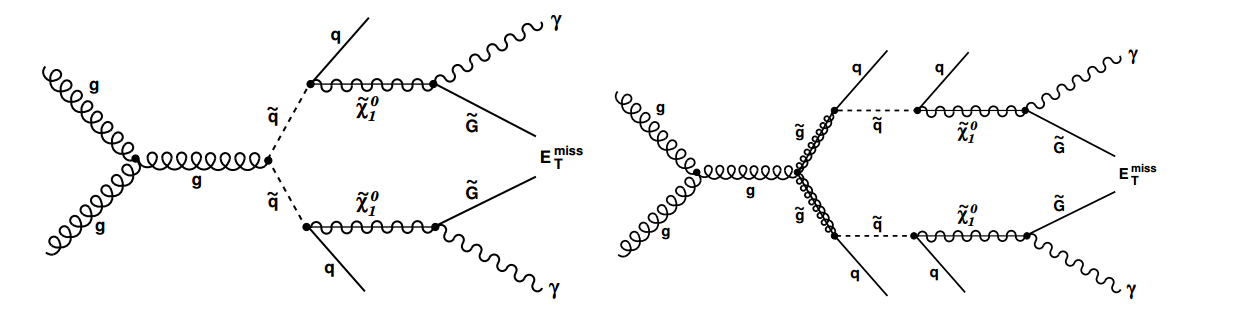
\includegraphics[width=\textwidth]{Feynman2.png}
\caption{Feynman diagram of $\widetilde{\chi}^0_1$ pair productions and $\widetilde{\chi}^0_1 \rightarrow \gamma + \widetilde{G}$ decay.}
\label{fig:feynman}
\end{figure}
\\
Here the neutralino $\widetilde{\chi}^0_1$ is the Next To Lightest SUSY Particle (NLSP) while the gravitino is the Lightest SUSY Particle (LSP). We search for a signature of a photon with significant impact parameter (defined below) in association with missing transverse energy $E^{\textrm{miss}}_T$ (MET) from the invisible gravitinos. Because we are assuming a conservation of $R$-parity, the neutralino must decay into the stable gravitino. The lifetime of the neutralino is not known (free parameter) but if we assume it to be large enough, it is possible to reconstruct photons that do not originate from the interaction vertex, signalling this SUSY event. We use photons that undergo a conversion into $e^+e^-$ pairs in the tracker. The tracks of the electrons and positrons can be precisely reconstructed and used to calculate the photon trajectory.

The data is collected by the CMS detector at the LHC using proton-proton collisions at a center-of-mass-energy of 8 TeV in 2012. The data corresponds to an integrated luminosity of 19.3 fb$^{-1}$\footnote{\href{https://twiki.cern.ch/twiki/bin/view/CMSPublic/LumiPublicResults\#2012\_Proton\_Proton\_Collisions}{Link}}. The analysis strategy is to start with a diphoton in the final state, then examine the impact parameter of every single photon for the displaced photon signal. $E^{\textrm{miss}}_T$ and the presence of jets are also required. The result will be an upper limit to the cross section for pair-production of $\widetilde{\chi}^0_1$s, each of which decays into a photon and invisible particles, and will be set as a function on $\widetilde{\chi}^0_1$ lifetime of which we will generate a number of samples.


\section{Photon Conversion Method: Impact Parameter}
\label{sec:IP}
As mentioned in section \ref{sec:intro} one must construct a main search variable. This variable is described in the following.\\
\\
The CMS Tracker based on silicon technology was designed to provide robust and precise reconstruction of charged-particle momenta in the high occupancy environment of LHC collisions. This inevitably led to a substantial amount of tracker material. The direct consequence is that a large fraction of photons convert into $e^+e^-$ pairs while traversing the tracker material. These are called \emph{photon conversions}. \\
\\
Considering the case that photons from $\widetilde{\chi}^0_1$ convert into $e^+e^-$ pairs in the CMS tracker, the photon conversion reconstruction can obtain the positions of the conversion vertices, as well as the photon directions from the $e^+e^-$ pairs. The latter is something a regular photon reconstruction cannot.  By extrapolating along the momentum direction from the conversion vertex back to the beam line, we can calculate the impact parameter of the displaced photons (figure \ref{fig:conversion}). The conversion reconstruction method has already been used so far in several physics applications \cite{PhysRevD.84.052011}.
\\
\\
\begin{figure}
\centering
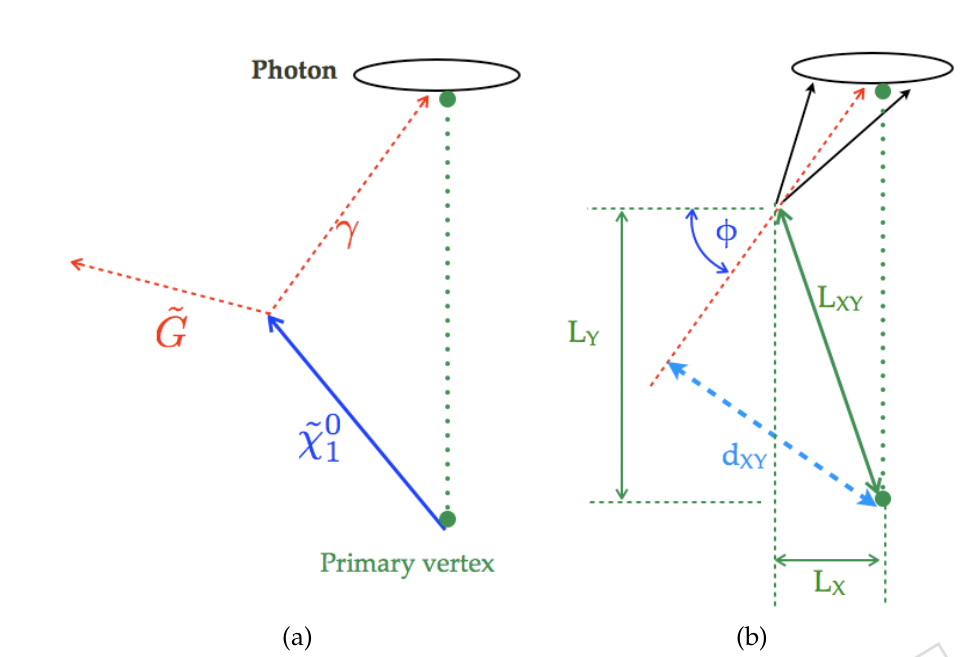
\includegraphics[width=10cm]{conversion.png}
\caption{(a): $\widetilde{\chi}^0_1 \rightarrow \gamma + \widetilde{G}$ view in the CMS tracker (b) the photon converts into $e^+e^-$ pairs allowing to reconstruct the impact parameter.}
\label{fig:conversion}
\end{figure}
\noindent The transverse impact parameter $d_\textrm{XY}$ is the distance of closest approach of the photon trajectory to the beamline in the transverse plane. It is the minimal distance a $\widetilde{\chi}^0_1$ would have travelled before decaying. The longitudinal impact parameter $d_\textrm{Z}$ is the distance from the chosen primary vertex and $z$ position where $d_\textrm{XY}$ is calculated (equation \ref{eq:dxy}). The photon trajectory is defined as a straight line from conversion vertex along the conversion momentum.

\begin{equation}
\begin{split}
d_{XY} &= -L_X \cdot \sin \phi + L_Y \cdot \phi \\
d_Z &= L_Z - \frac{L_X \cdot p_X + L_Y \cdot p_Y}{p_T} \cdot \frac{p_Z}{p_T}
\label{eq:dxy}
\end{split}
\end{equation}
where $L$ is the vector between the conversion vertex and the primary vertex, and the $\phi$ angle is the polar angle of the conversion momentum vector $p$ in azimuth, which is calculated by the vector summation of $e^+e^-$ pair momenta at the conversion vertex.\\
\\
\noindent In the high luminosity conditions, multiple collisions give multiple primary vertices. The longitudinal Impact Parameter (IP) $d_Z$ will not be used as it has to account for this spread. We will focus on $d_{XY}$ as the main search variable. The primary vertex is chosen by selecting the minimal $\chi^2$-probability in every single event.\\
\\

\noindent As explained above, the impact parameter (IP) of a photon (equation \ref{eq:dxy}) is calculated w.r.t. the primary vertex, by extrapolating the conversion momentum from the conversion vertex. In the decay of $\widetilde{\chi}^0_1 \rightarrow \gamma + \widetilde{G}$, the non-zero IP of the photon indicates the non-zero $\widetilde{\chi}^0_1$ lifetime. The reconstructed $\gamma$ $d_{XY}$ distributions from different $\widetilde{\chi}^0_1$ lifetimes in MC samples is shown in figure \ref{fig1:dxy}. We see that for low $\widetilde{\chi}^0_1$ lifetimes the $d_{XY}$ variable is not sensitive. One therefore wants to aim for longer living particles. However, if a neutralino has a very long lifetime a substantial amount of these particles will escape our detector. Therefore, only a limited range of useable neutralino lifetimes is present. The range used in this analysis runs from $c\tau = 1$ to 50 cm, where $c$ is the speed of light and $\tau$ the lifetime.

\begin{figure}[h]
\begin{subfigure}[h]{8cm}
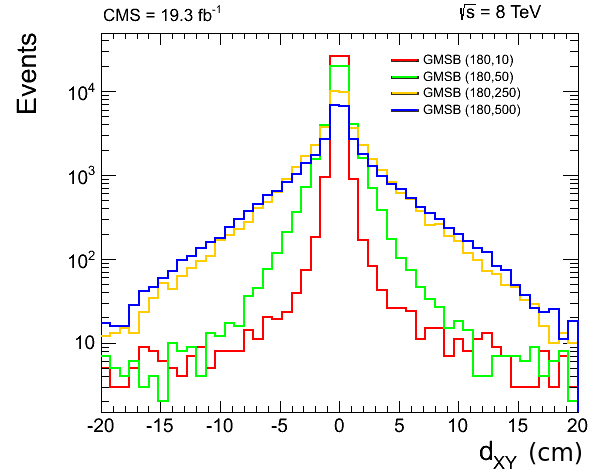
\includegraphics[width=\textwidth]{dxycomparisonsignal.png}
\end{subfigure} \hspace{9mm}
\hspace{-1cm}
\begin{subfigure}[h]{8cm}
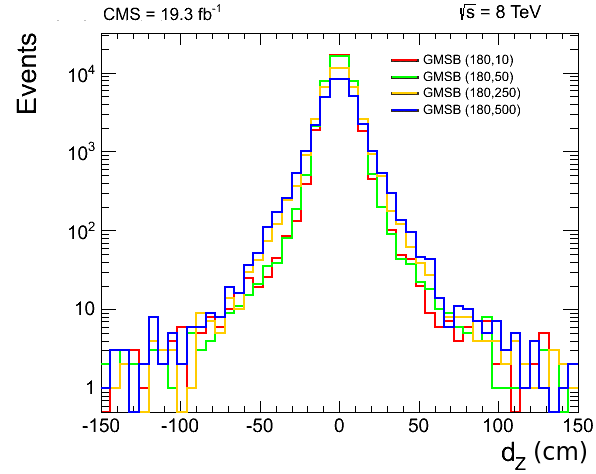
\includegraphics[width=\textwidth]{dzcomparisonsignal.png}
\end{subfigure}
\caption{\small Reconstructed $\gamma$ impact parameter from long lived $\widetilde{\chi}^0_1 \rightarrow \gamma + \widetilde{G}$ decay. \emph{Left: }transverse. \emph{Right: }longitudinal.}
\label{fig1:dxy}
\end{figure}
As previously mentioned, in pile-up conditions multiple collisions give multiple primary vertices. The true primary vertex has a large divergence in the longitudinal direction, but luckily much less in the transverse direction. It is for this reason that the transverse IP and not the longitudinal IP is used in this analysis.

It should already be clear to the reader that because of the very low cross section of our signal sample it will prove to be difficult to find a region where we can distinguish signal from background. Indeed, an interaction with a low cross section inherently means that not many of these events will occur and other interations that occur much more frequently have the chance in giving non-zero contributions to our main search variable. The main reason for this is the non-perfect performance of the detector. It can occur that particles are misidentified leading to a wrong event reconstruction that can give these non-zero contributions. 


The interaction that is being studied (see figure \ref{fig:feynman}) will have certain physical characteristics. For example, we expect there to be multiple jets present, so removing events that have only one or zero jets will reduce the background whereas the signal will be less affected. This will be made more clear by the $n-1$ cuts in figures figures \ref{fig:n-1photpt} and \ref{fig:n-1njets}.




\chapter{Analysis Technique}
\label{ch:analysis}
This chapter begins by highlighting the physical phenomena in our events of interest in section \ref{sec:eventsel}. The background was estimated using a data/Monte Carlo comparison and a data-driven method which are explained in sections \ref{sec:dataMC} and \ref{sec:background} respectively. Section \ref{sec:sysunc} elaborates more on the systematic uncertainties and section \ref{sec:resultsandint} summarizes our results.

\section{Event Selection}
\label{sec:eventsel}
The data were recorded using the CMS two-level trigger system. This analysis selects events with at least two photons. A diphoton trigger is required with ECAL transverse energy thresholds $E_T$ set to a value of 40 GeV for the leading photon. This ensures being on the plateau of the trigger efficiency, the offline analysis selects events with at least two photons in the event with $E_T > 50$ GeV.\\
\\
 As the previous analysis already excluded up to a $\Lambda$ of 140 TeV\footnote{More information can be found in section \ref{sec:GMSB}.}, this analysis is based on a $\Lambda$-value of 180 TeV which corresponds to a lower cross section of only 0.0145 pb and a $\widetilde{\chi}^0_1$ mass of 256.8 GeV. The higher luminosity of the 2012 dataset should make it possible to probe at lower cross sections than the 2011 dataset. This means that the only remaining free variable is the $\widetilde{\chi}^0_1$ lifetime, which is determined by the parameter $C_\textrm{grav}$. The different lifetimes are listed in Table \ref{table:lifetimes}.

\begin{table}[h]
\centering
\caption{List of the used $\chi^0_1$ lifetimes in this analysis.}
\begin{tabular}{c|c|c}
\hline
$\Lambda$ [TeV] & c$\tau$ [cm] & $\sigma$ [pb] \\
\hline
180 & 1, 5, 25, 50 & 0.0145\\
\hline
\end{tabular}
\label{table:lifetimes}
\end{table}

\noindent Because of the high luminosity during the run, many events had multiple proton-proton interactions (called ``pile-up''), leading to a distribution of primary vertices. The pile-up conditions at high luminosity affect the event selections, in particular conversion reconstruction efficiencies. The generated pile-up distribution in the Monte Carlo samples was reweighted.\\
\\
It is also notable to mention that apart from the decay into a photon $\widetilde{\chi}^0_1 \rightarrow \gamma + \widetilde{G}$ there is a corresponding decay into a $Z$-boson $\widetilde{\chi}^0_1 \rightarrow Z + \widetilde{G}$. The branching ratio in the GMSB model between these two is determined by the parameter $\Lambda$. We will only select events that correspond to the former decay.\\
\\
In the Monte Carlo simulation, signal photons are found to be mainly in the ECAL barrel region with high transverse energy $E_T$. The decay model also predicts multiple reconstructed high energy jets, as well as a large value of missing transverse energy $E^\textrm{miss}_T$.\\

Because of the single $\gamma$ and jets in the final state (see fig \ref{fig:feynman}), the backgrounds are

\begin{itemize}
\item \textbf{$\gamma$-plus-jets:} a real $\gamma$ together with a jet that can be mistagged as a photon.
\item \textbf{QCD multi-jets:} two jets can now be mistagged as two photons. The probability of two jets to be mistagged as photons is small but because there is such a huge QCD-event production, the background is substantial enough te be taken into account.
\item \textbf{$\mathbf{t\bar{t}}$-jets:} the top quark can decay semileptonically ($t \rightarrow Wb \rightarrow l \nu_l b$) and the lighter lepton is mistagged as a photon together with a jet being misinterpreted as a photon. We expect this background to be neglegible.
\end{itemize}
We have to select our events in such a way that we cut away as much background as possible while leaving the highest amount of signal. This is illustrated in the so-called $n-1$ plots in figures \ref{fig:n-1photpt} and \ref{fig:n-1njets}. $n-1$ plots show the distribution of a variable where all the cuts ($n$) are implemented except for the cut on the concerned variable ($n-1$). Although, because we are dealing with very low statistics in our analysis, the cut on the number of photons is discarded. The signal sample used has a lifetime with $c\tau = 50$ cm.\\
\\

\begin{figure}[H]
\begin{subfigure}[h]{8cm}
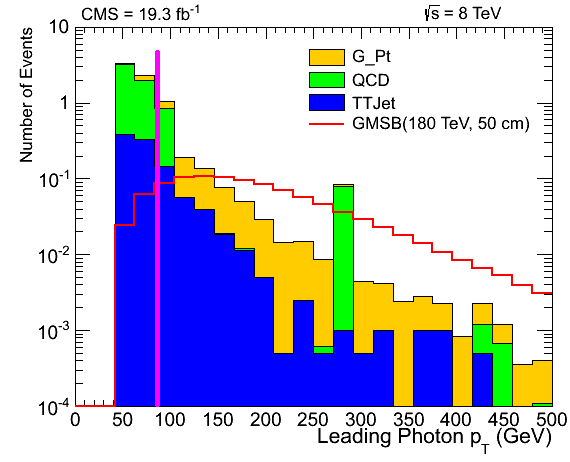
\includegraphics[width=\textwidth]{n-1PhotPtline.png}
\end{subfigure}
\begin{subfigure}[h]{8cm}
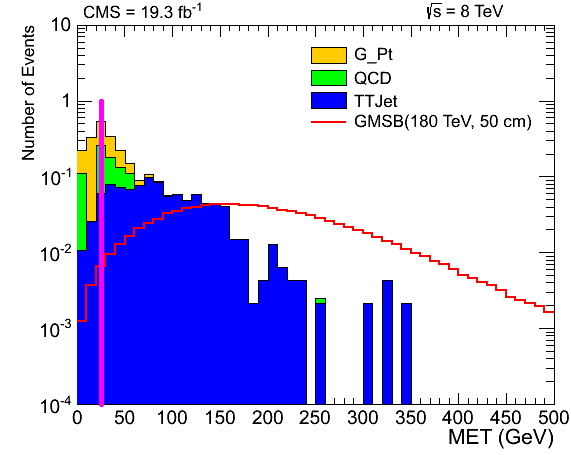
\includegraphics[width=\textwidth]{n-1METline.png}
\end{subfigure}
\caption{$n-1$ plot of the leading jet $p_T$ (\emph{left}) and $E^\textrm{miss}_T$ (\emph{right}). The purple line indicates where the cut was impemented.}
\label{fig:n-1photpt}
\end{figure}

\vspace{-0.2cm}

\begin{figure}[H]
\begin{subfigure}[h]{8cm}
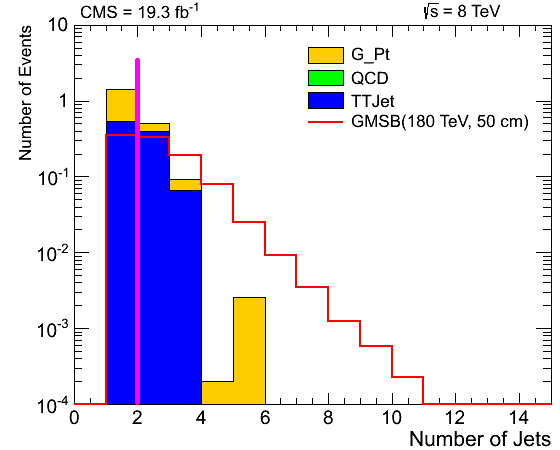
\includegraphics[width=\textwidth]{n-1nJetsline.png}
\end{subfigure}
\begin{subfigure}[h]{8cm}
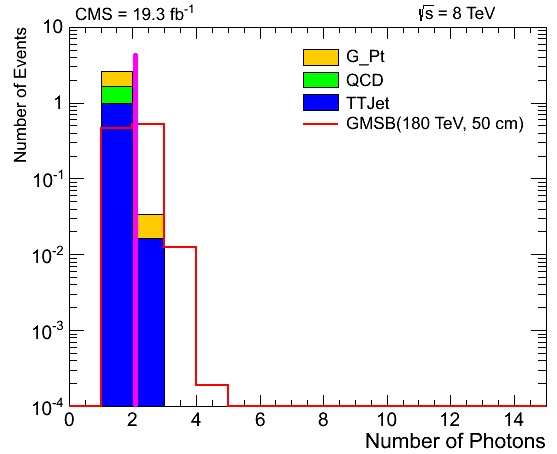
\includegraphics[width=\textwidth]{n-1nPhotline.png}
\end{subfigure}
\caption{$n-1$ plot of the number of jets (\emph{left}) and number of photons (\emph{right}). The purple line indicates where the cut was impemented.}
\label{fig:n-1njets}
\end{figure}


The unconverted and converted photon candidates are reconstructed from clusters of energy in the ECAL. At least one photon candidate with transverse $E_T > 50$ GeV and reconstructed in the ECAL barrel region is required. The transverse distribution of energy in the associated cluster of ECAL crystals must be consistent with that expected from a photon, and the energy detected in the HCAL behind the photon shower cannot exceed 5\% of the ECAL energy. Events originating from decaying heavy particles as the ones we are looking for are characterised by isolated photons. To look for these isolated photons, we use official CMS search criteria. We look at a cone around the photon with a $\Delta R < 0.3$ ($\Delta R = \sqrt{(\Delta \eta)^2 + (\Delta \phi)^2}$) (see figure \ref{fig:cone}). The pseudorapidity $\eta$ is a variable that indicates if the particle in question is travelling in a direction perpendicular to the beam, in parallel or something in between. It is defined as:
\begin{equation}
\eta = -\ln\left[\tan\left(\frac{\theta}{2}\right)\right]
\end{equation}
where $\theta$ is the polar angle with respect to the counter clockwise beam direction and goes from 0 (perpendicular) to $\infty$ (longitudinal).
\\
\begin{figure}[h]
\centering
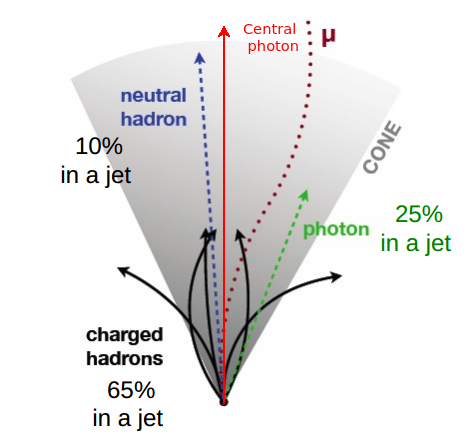
\includegraphics[width=8cm]{cone.png}
\caption{Example of particles that can accompany a photon. We look at particles that are close to the photon, within a cone-like shape.}
\label{fig:cone}
\end{figure}
\\
The following photon isolation criteria are used to select these ``good photons'':


\begin{itemize}
\item $\sum E^\textrm{Charged hadron}_T < 2.6$ GeV
\item $\sum E^\textrm{Neutral hadron}_T < 3.5 + 0.04 \cdot E^\textrm{Central photon}_T$ GeV
\item $\sum E^\textrm{Other photons}_T < 1.3 + 0.004 \cdot E^\textrm{Central photon}_T$ GeV
\end{itemize}

\begin{itemize}
\item $\sigma_{i\eta i\eta} < 0.012$;
\item $H/E <$ 0.05;
\end{itemize}

where $H/E$ has been defined as the sum of the energies of HCAL towers within a cone of size $\Delta R<0.15$ centred on the supercluster position, divided by the supercluster energy\footnote{More information can be found in this \href{https://twiki.cern.ch/twiki/bin/viewauth/CMS/HoverE2012}{\textcolor{blue}{link}}.}. $\sigma_{i\eta i\eta}$ is a measure of the transverse profile of the shower.\\
\\
In the ideal situation, two to four jets are expected for neutralino pair-production as illustrated in figure \ref{fig:feynman}. However, considering the jet reconstruction efficiency and energy resolution, at least two jets with $\eta \leq 2.4$ with $p_T > 35$ GeV are required.
\\
\\
If a $\widetilde{\chi}^0_1 \rightarrow \gamma + \widetilde{G}$ decay were to occur, one expects a $\gamma$ that signals a rather large impact parameter together with large $E^\textrm{miss}_T$ from the invisible $\widetilde{G}$. So, as already explained frequently in this analysis, $E^{miss}_T$ is an important parameter indicating the difference between signal and background. As is motivated in the 7 TeV analysis \cite{Hongliang}, a cut of $E^{miss}_T > 30$ GeV for the signal selection is set in order to eliminate most of the background and keep the signal efficiency.\\
\\
Because it is possible that an electron deposits its energy in the calorimeter and fakes either a photon or a conversion, these events are now be vetoed out with the help of some well chosen cuts. We motivate this choice with the help of figure \ref{fig:matchedele}. It is clear that when we veto the events where a conversion or a photon matches an electron, these background events will reduce as many more electrons fake a conversion or a photon in the $t\bar{t}$-jets background (this is also the reason why it is a background). The figure shows that the ratio of this matching to no matching is much higher for the $t\bar{t}$-jets background than for the signal sample. Therefore, more background than signal events will be vetoed out.


\begin{center}
\begin{figure}[tb]
\begin{subfigure}[h]{8cm}
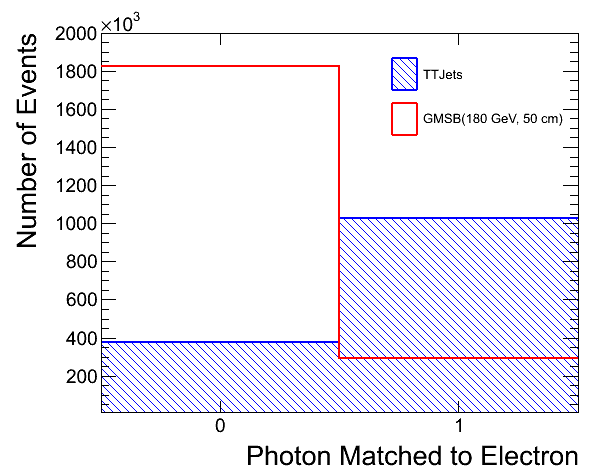
\includegraphics[width=\textwidth]{phomatchedele.png}
\end{subfigure}
\begin{subfigure}[h]{8cm}
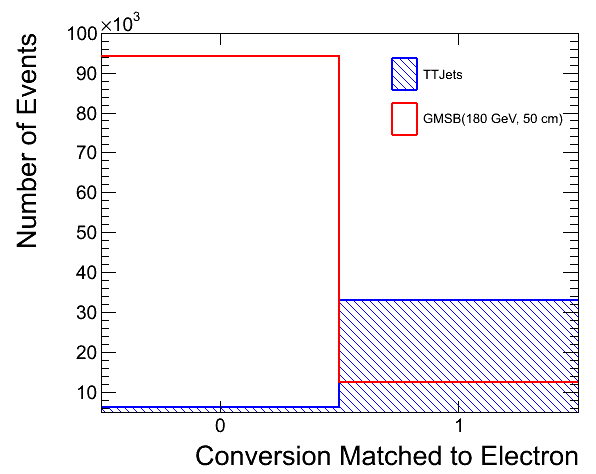
\includegraphics[width=\textwidth]{convmatchedele.png}
\end{subfigure}
\caption{\emph{Left: }Difference in the new boolean variable that matches a photon to an electron (0 for false, 1 for true). \emph{Right: }Difference in the new boolean variable that matches a conversion to an electron (0 for false, 1 for true).}
\label{fig:matchedele}
\end{figure}
\end{center}

\section{Data/MC comparison}
\label{sec:dataMC}
For a first background determination, we started by trying to get a data/Monte Carlo (MC) comparison. The agreement should not be perfect because the QCD/$\gamma$+jets modelling are known to be sub-optimal and the QCD MC statistics are also very low. This is illustrated in figures \ref{fig:nphotandnjetMC} to \ref{fig:dxyMC}. S$_\textrm{Minor}$ is the minor axis of the ellipse from the energy deposit in the ECAL. $\sigma_{i\eta i\eta}$ is a measure of the transverse profile of the shower. Its properties are used to ensure that the candidate is consistent with the shape expected from a photon.

\vspace{-4mm}

\begin{center}
\begin{figure}[H]
\begin{subfigure}[h]{8cm}
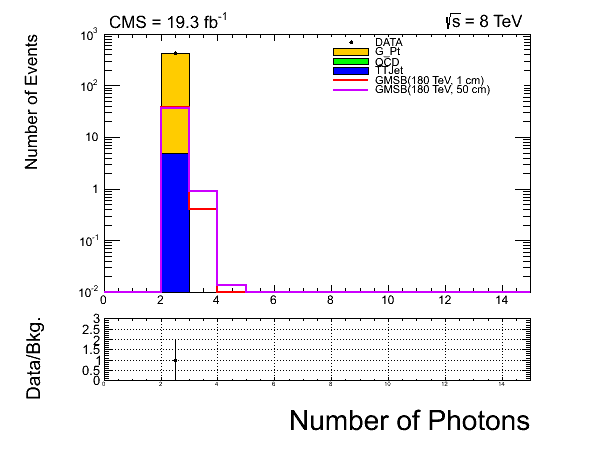
\includegraphics[width=\textwidth]{nPhotMC.png}
\end{subfigure}
\hspace{-9mm}
\begin{subfigure}[h]{8cm}
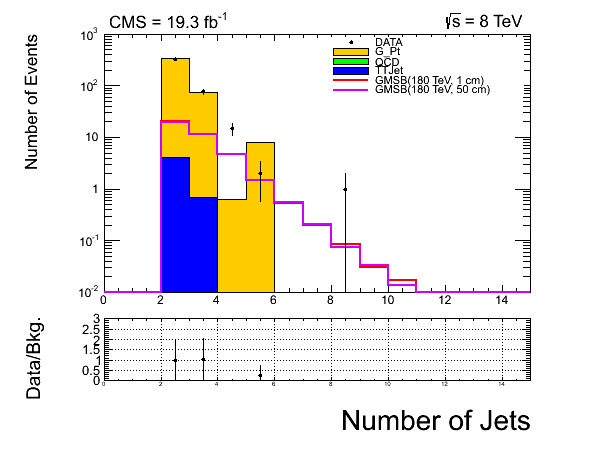
\includegraphics[width=\textwidth]{nJetsMC.png}
\end{subfigure}
\caption{\small Data/MC comparison for the number of photons (\emph{left}) and number of jets (\emph{right}). Two signal samples with $\Lambda = 180$ TeV and $c\tau = 1$ and 50 cm are also shown.}
\label{fig:nphotandnjetMC}
\end{figure}
\end{center}

\vspace{-16mm}

\begin{center}
\begin{figure}[H]
\begin{subfigure}[h]{8cm}
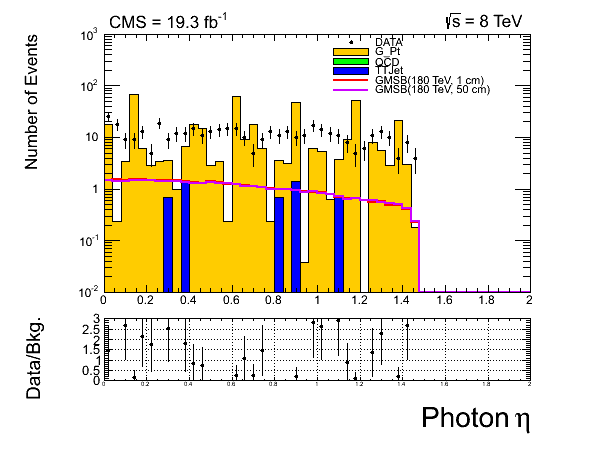
\includegraphics[width=\textwidth]{EtaMC.png}
\end{subfigure}
\hspace{-9mm}
\begin{subfigure}[h]{8cm}
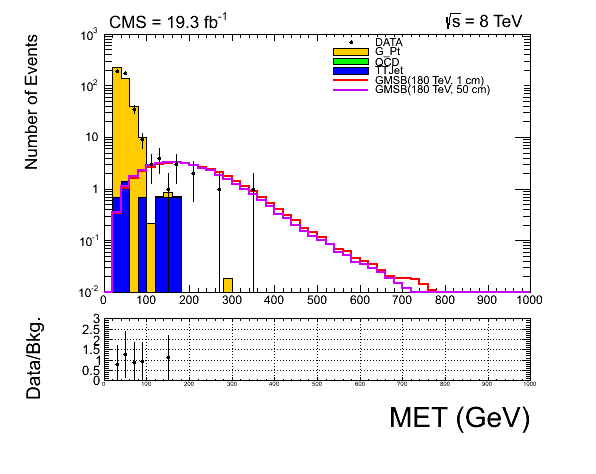
\includegraphics[width=\textwidth]{METMC.png}
\end{subfigure}
\caption{\small Data/MC comparison for $\eta$ (\emph{left}) and $E^\textrm{miss}_T$ (\emph{right}). Two signal samples with $\Lambda = 180$ TeV and $c\tau = 1$ and 50 cm are also shown.}
\label{fig:etaandmetMC}
\end{figure}
\end{center}


\begin{center}
\begin{figure}[H]
\begin{subfigure}[h]{8cm}
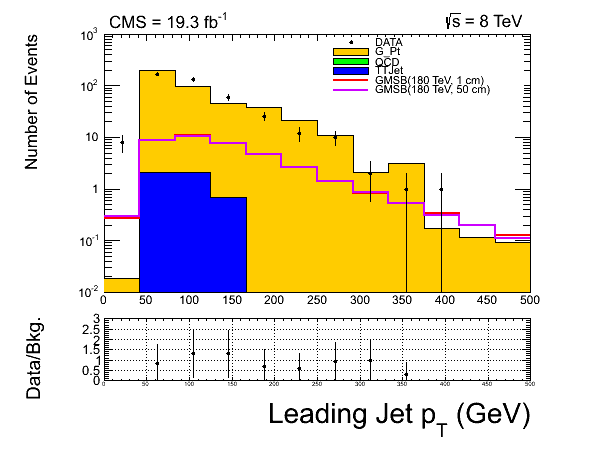
\includegraphics[width=\textwidth]{JetPtleadingMC.png}
\end{subfigure}
\hspace{-9mm}
\begin{subfigure}[h]{8cm}
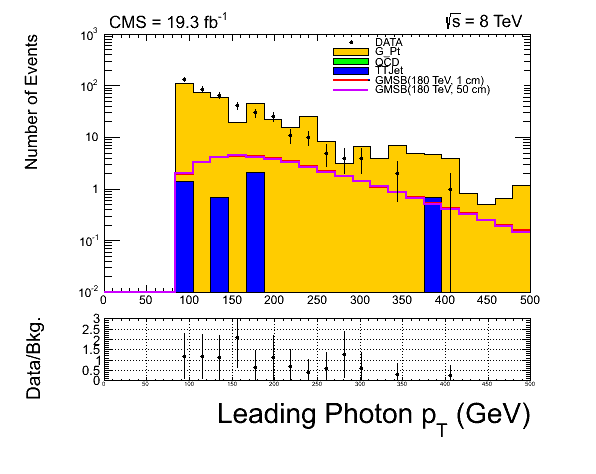
\includegraphics[width=\textwidth]{PhotPtleadingMC.png}
\end{subfigure}
\caption{\small Data/MC comparison for $p_T$ of the leading jet (\emph{left}) and $p_T$ of the leading photon (\emph{right}). Two signal samples with $\Lambda = 180$ TeV and $c\tau = 1$ and 50 cm are also shown.}
\label{fig:jetandphotptMC}
\end{figure}
\end{center}

\vfill

\begin{center}
\begin{figure}[H]
\begin{subfigure}[h]{8cm}
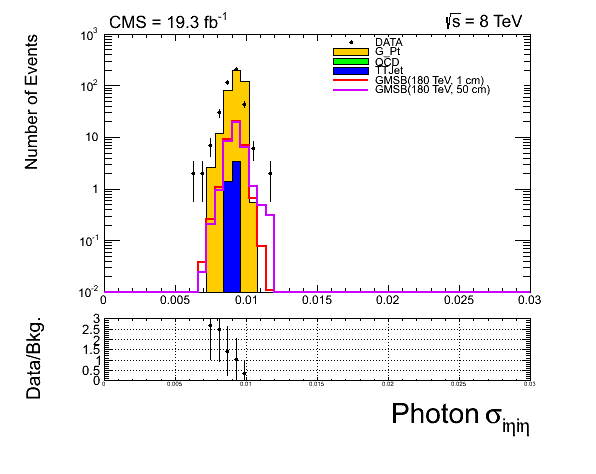
\includegraphics[width=\textwidth]{sigmaietaMC.png}
\end{subfigure}
\hspace{-9mm}
\begin{subfigure}[h]{8cm}
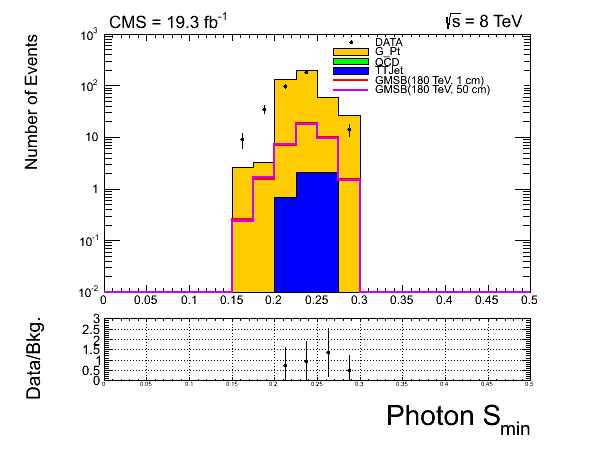
\includegraphics[width=\textwidth]{sMinMC.png}
\end{subfigure}
\caption{\small Data/MC comparison for $\sigma_{i \eta i \eta}$ (\emph{left}) and S$_\textrm{Minor}$ (\emph{right}). Two signal samples with $\Lambda = 180$ TeV and $c\tau = 1$ and 50 cm are also shown.}
\label{fig:sigmaietaandsminMC}
\end{figure}
\end{center}


\begin{center}
\begin{figure}[H]
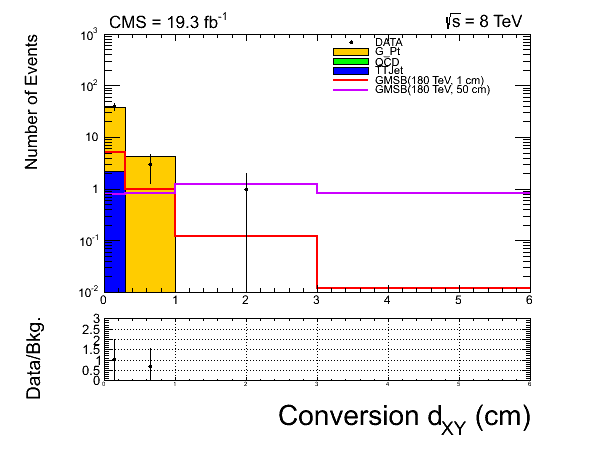
\includegraphics[width=\textwidth]{dXYMC.png}
\caption{\small Data/MC comparison for $d_{XY}$. Two signal samples with $\Lambda = 180$ TeV and $c\tau = 1$ and 50 cm are also shown.}
\label{fig:dxyMC}
\end{figure}
\end{center}


From these figures we see that the data/MC comparison is far from ideal but it's the best we could do. However, some important conclusions can be made:
\begin{itemize}
\item The main backgrounds are not well modelled in Monte Carlo.
\item The $\gamma$+jets is our main background and the QCD-jets and $t\bar{t}$-jets are almost negligible.
\item The $E^\textrm{miss}_T$ does not depend on the $\widetilde{\chi}^0_1$-lifetime (which is expected).
\item The signal region is in the high $E^\textrm{miss}_T$ tail.
\end{itemize}



The main search variable $d_{XY}$ is shown in figure \ref{fig:dxyMC}. These results were presented to the Long Lived group in CMS. Because we encountered the need of at least two photons in our events, one of the comments was to try the di-photon trigger instead of the single photon trigger that was used up to now. This would allow us to lower the thresholds on the photon $p_T$ and give us more useful data. Essentially this meant for us to change the code to run on AOD (Analysis Object Data) instead of RECO (Reconstructed data).

\section{Background Determination}
\label{sec:background}

We can see from figures \ref{fig:nphotandnjetMC} to \ref{fig:dxyMC} that the MC does not model the data very well. This is both due to a lack of MC statistics and known mis-modelling effects (for QCD and $\gamma$+jets) due to large uncertainties on the cross section etc. However, they are reasonable enough to conclude that our key variables are understood both in data and MC. For $t\bar{t}$-bar, since this is a negligible background (less than 1\%), we estimate this using MC scaled to luminosity. For $\gamma$+jets we estimate the shape and normalisation using a data driven approach, which will be explained in this section.\\
\\
The data-driven background determination is a strategy for estimating the QCD and $\gamma$+jets background via data control samples that are kinematically similar to the candidate sample while having no real $E^\textrm{miss}_T$ (remember that this parameter is expected to be high in the signal region). In the main backgrounds, the single-$\gamma$-plus-jets events and QCD mulit-jets events, the jets can be misidentified as photons and are called \emph{fake photons}. These fake photons have to fail at least one of the photon isolation requirements that are given in section \ref{sec:eventsel}.
\\
\\
Indeed, the $\widetilde{\chi}^0_1 \rightarrow \gamma + \widetilde{G}$ decay has two signatures: $E^\textrm{miss}_T$ from $\widetilde{G}$ and large transverse IP from the displaced photons. Therefore the $\widetilde{\chi}^0_1$ signal has large $E^\textrm{miss}_T$, while the main background (single $\gamma$-plus-jets and QCD multi-jets) has small $E^\textrm{miss}_T$ with tails extending to high $E^\textrm{miss}_T$. We construct a control region of low $E^\textrm{miss}_T$ and use this control region to estimate the background in the search/signal region, by measuring the $d_{XY}$ distribution. 
Summarized, we get:

\begin{enumerate}
\item The background is more prominent than the signal in the region of low $E^{miss}_T$.
\item The data in the region of low $E^{miss}_T$ is therefore made up almost entirely of background events.
\item The background should not depend on the $E^{miss}_T$ as no prominent invisible particles are involved.
\item The data is separated into a background region (with low $E^\textrm{miss}_T$) and a signal region (with high $E^\textrm{miss}_T$).
\item The data in the background region can be used in the signal region because of 3.
\end{enumerate}

In this analysis, we define $E^\textrm{miss}_T < 20$ GeV as the background control region, and the $E^\textrm{miss}_T > 30$ GeV as the signal region. In figure \ref{fig:dxycomparison} we can see that, with a proper normalization, background events (fake photons) do not depend on the $E^{miss}_T$ (point 3 in the above). Control regions 1 and 2 have similar shapes. We can also see that data in the low $E^\textrm{miss}_T$ region can be used to estimate the background in the signal region. The background is normalized to the total number of events in the data sample.\\
\\
After performing the validation checks for the data-driven method we used this estimation for figures \ref{fig:nphotandnjetDD} to \ref{fig:jetandphotleadDD}. The background in the $d_{XY}$ variable was scaled using the peak of the distribution in data. This is necessary to be non-biased for possible signal events in the tail.


\begin{figure}[htb]
\centering
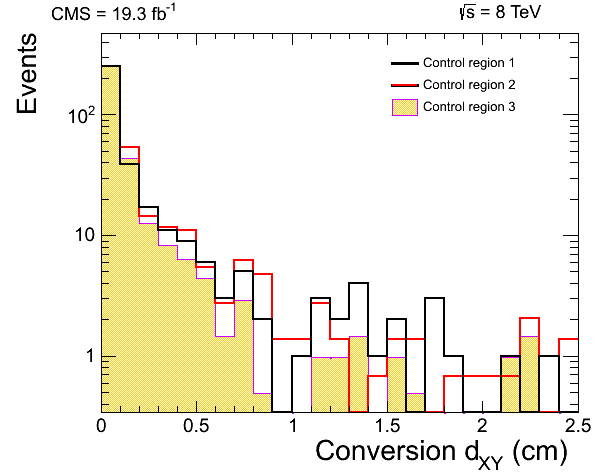
\includegraphics[width=\textwidth]{dxycomparisonfakehighfakelowisolow.png}
\caption{The shape of the fake photons (real background) in the high $E^\textrm{miss}_T$ (control region 1) is the same as the shape of fake photons in the low $E^\textrm{miss}_T$ (control region 2) and as the shape of real photons in the  the low $E^\textrm{miss}_T$ (control region 3).}
\label{fig:dxycomparison}
\end{figure}


\vspace{-8mm}

\begin{center}
\begin{figure}[H]
\begin{subfigure}[h]{8cm}
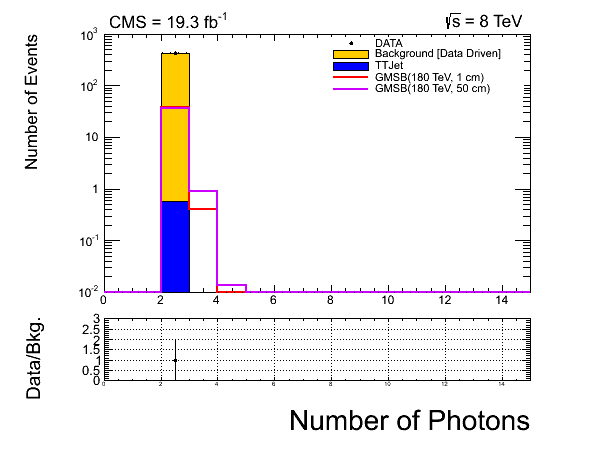
\includegraphics[width=\textwidth]{nPhotDD.png}
\end{subfigure}
\hspace{-9mm}
\begin{subfigure}[h]{8cm}
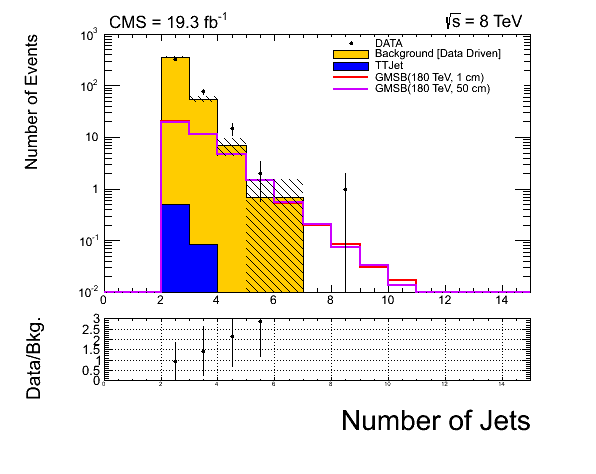
\includegraphics[width=\textwidth]{nJetsDD.png}
\end{subfigure}
\caption{\small The number of photons (\emph{left}) and number of jets (\emph{right}) using the data-driven background method. Two signal samples with $\Lambda = 180$ TeV and $c\tau = 1$ and 50 cm are also shown.}
\label{fig:nphotandnjetDD}
\end{figure}
\end{center}

\vspace{-20mm}

\begin{center}
\begin{figure}[H]
\begin{subfigure}[h]{8cm}
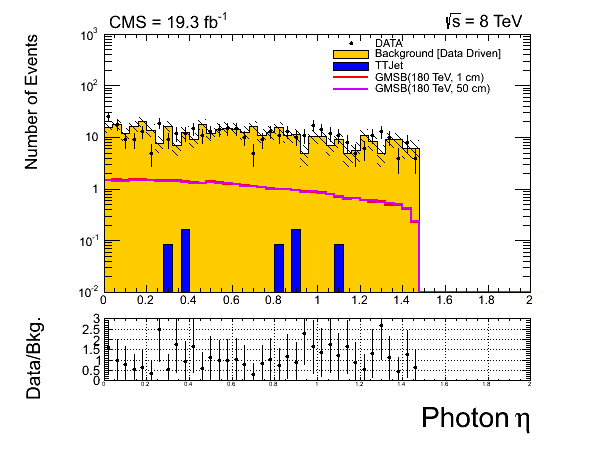
\includegraphics[width=\textwidth]{EtaDD.png}
\end{subfigure}
\hspace{-9mm}
\begin{subfigure}[h]{8cm}
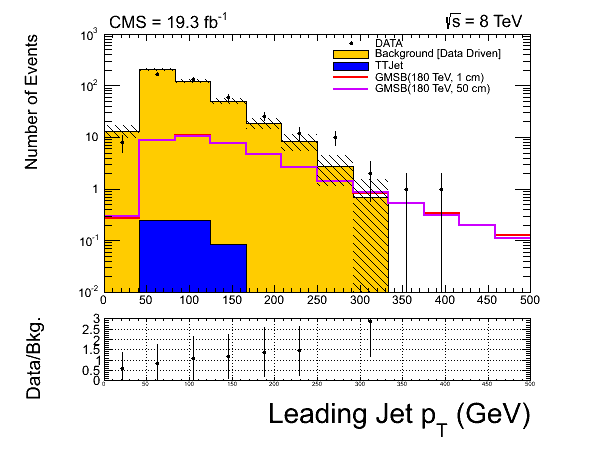
\includegraphics[width=\textwidth]{JetPtleadingDD.png}
\end{subfigure}
\caption{\small The photon $\eta$ (\emph{left}) and $p_T$ of the leading jet (\emph{right}) using the data-driven background method. Two signal samples with $\Lambda = 180$ TeV and $c\tau = 1$ and 50 cm are also shown.}
\label{fig:etaandmetDD}
\end{figure}
\end{center}

\vspace{-17mm}

\begin{center}
\begin{figure}[H]
\begin{subfigure}[h]{8cm}
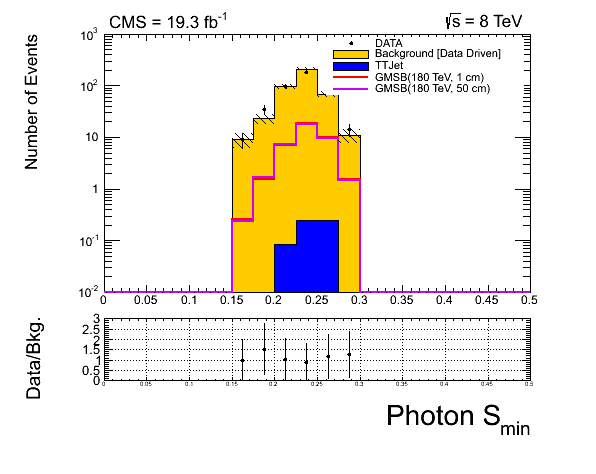
\includegraphics[width=\textwidth]{sMinDD.png}
\end{subfigure}
\hspace{-9mm}
\begin{subfigure}[h]{8cm}
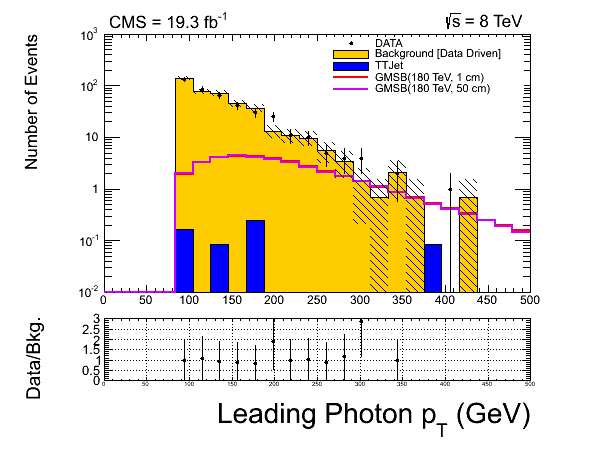
\includegraphics[width=\textwidth]{PhotPtleadingDD.png}
\end{subfigure}
\caption{\small The photon S$_\textrm{Minor}$ (\emph{left}) and $p_T$ of the leading photon (\emph{right}) using the data-driven background method. Two signal samples with $\Lambda = 180$ TeV and $c\tau = 1$ and 50 cm are also shown.}
\label{fig:jetandphotleadDD}
\end{figure}
\end{center}

\vspace{-17mm}

\begin{center}
\begin{figure}[H]
\begin{subfigure}[h]{8cm}
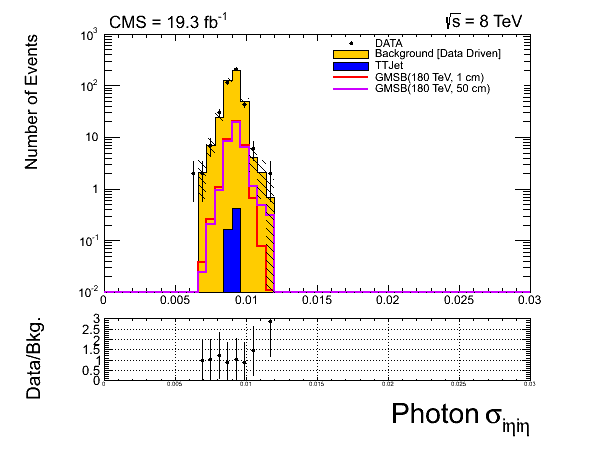
\includegraphics[width=\textwidth]{SigmaIetaDD.png}
\end{subfigure}
\hspace{-9mm}
\begin{subfigure}[h]{8cm}
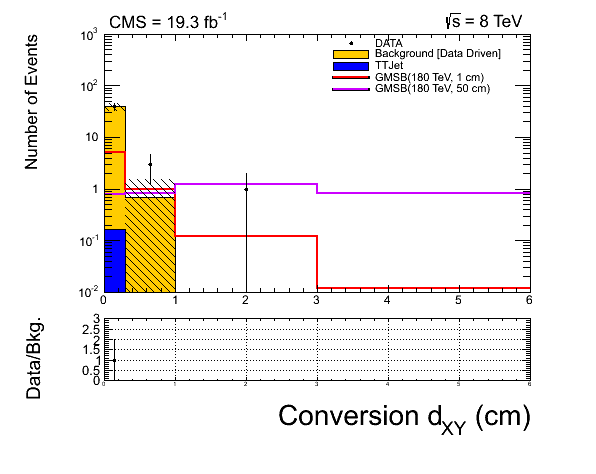
\includegraphics[width=\textwidth]{dXYDD.png}
\end{subfigure}
\caption{\small $\sigma_{i \eta i \eta}$ (\emph{left}) and $d_{XY}$ (\emph{right}) using the data-driven background method. Two signal samples with $\Lambda = 180$ TeV and $c\tau = 1$ and 50 cm are also shown.}
\label{fig:sigmaietaandsminDD}
\end{figure}
\end{center}

The full cut flow is summarized in table \ref{table:cutflow}. We clearly see that we start with a huge number of background with only a handful of signal events. The preselection includes several requirements such as a well defined interaction vertex, photons in the barrel region and photon isolation. The $E^\textrm{miss}_T$ differentiates between the signal region ($E^{miss}_T > 30$ GeV) and background region ($E^{miss}_T < 20$ GeV). When we select the number of photons that are necessary, other photon isolation requirements are also implemented.\\
\\
The final plot of the $d_{XY}$ conversion variable is shown in figure \ref{fig:sigmaietaandsminDD} (\emph{right}). Accounting for possible fluctuations in the data no excess in the tail is seen.

\begin{table}[h]
\scriptsize
\centering
\caption{Cutflow table of two signal samples with $c\tau = 50$ and 1 cm, the data-driven, $t\bar{t}$-bar and total background, the signal-over-background ratio and the data. We assumed systematic uncertainties of 10\% for signal and 30\% for the background.}
\begin{tabular}{|c|c|c|c|c|c|c|c|}
\hline
& GMSB & GMSB & \multirow{2}{*}{Bkg.[DD]} & \multirow{2}{*}{TTJet} & \multirow{2}{*}{Total Bkg} & \multirow{2}{*}{$\frac{S}{\sqrt {B}}$} & \multirow{2}{*}{Data} \\
&(180,50) & (180,1) & &  & & &  \\
\hline
All & $280 \pm 28$ & $280 \pm 28$ & $2.2 \cdot 10^{12}$ & $2.6 \cdot 10^{5}$ & $(2.2 \pm 0.7) \cdot 10^{12}$ & $2 \cdot 10^{-4}$ & $2.2 \cdot 10^{12}$\\
Presel. & $174 \pm 17$ & $179 \pm 18$ & $7.1 \cdot 10^{10}$ & $8.5 \cdot 10^{3}$ & $(7.2 \pm 2.2) \cdot 10^{10}$ & $2 \cdot 10^{-4}$ & $7.2 \cdot 10^{10}$\\
$E^\textrm{miss}_T$ $^\ast$ & $171 \pm 17$ & $177 \pm 18$ & $5\cdot 10^{10}$ & $7.7 \cdot 10^{3}$ & $(5.0 \pm 1.5) \cdot 10^{10}$ & $8 \cdot 10^{-4}$ & $5.0 \cdot 10^{10}$\\
No. jets$\geq 2$ & $92 \pm 9$ & $95 \pm 10$ & $3.2 \cdot 10^{9}$ & $3.9 \cdot 10^3$ & $(3.2 \pm 1) \cdot 10^{9}$ & $2 \cdot 10^{-3}$ & $2.1 \cdot 10^{9}$\\
No. $\gamma\geq 2$ & $40 \pm 4$ & $40 \pm 4$ & $2.1 \cdot 10^7$ & 0.02 & $(2.1 \pm 0.6) \cdot 10^7$ & 0.01 & $1.3 \cdot 10^7$\\
No. conv.$\geq 1$ & $4 \pm 0.4$ & $6 \pm 0.6$ & 40 & 0.02 & $40 \pm 12$ & 0.58 & 43\\
\hline
\end{tabular}
$^\ast$We differentiate between the signal region ($E^{miss}_T > 30$ GeV) and background region ($E^{miss}_T < 20$ GeV).
\label{table:cutflow}
\end{table}

\section{Systematic Uncertainties}
\label{sec:sysunc}
The uncertainty in the luminosity determination is 2.2 \% \cite{CMS-PAS-SMP-12-008}. The sources of systematic uncertainty affecting the signal acceptance are the following. The calorimeter response to different types of particles is not perfectly linear and hence corrections are made to properly map the measured jet energy deposition. The uncertainty on this correction is referred to as the uncertainty on the jet energy scale and varies as a function of position and transverse momentum of the jet. A similar uncertainty on the photon energy scale in the barrel is also present. Due to time constraints there was not enough time to compute all the systematic uncertainties. Therefore we made an educated assumption on the systematic uncertainty (10\%) and the background (30\%). These uncertainties are propagated unto table \ref{table:cutflow} and figures \ref{fig:nphotandnjetDD} to \ref{fig:sigmaietaandsminDD}. These uncertainties will be computed properly in the near future.

\section{Results and Interpretation}
\label{sec:resultsandint}
The observed event yield in data is consistent with the SM background prediction, and upper limits are obtained on the production cross section of a long-lived neutralino in the context of the the SPS8 model of GMSB supersymmetry, assuming $\mathcal{B}\left(\widetilde{\chi}^0_1 \rightarrow \gamma \widetilde{G} \right) = 100\%$. Exclusion limits are computed with a modified frequentist CL$_\textrm{s}$ method \cite{CMS-NOTE-2011-005,Junk:1999kv,0954-3899-28-10-313}\footnote{See further.}, using the asymptotic approximation for the test statistic as described in reference \cite{lalala}. These results are shown in figures \ref{fig:limitplotsnoshape}, where we used a cut and count approach, and \ref{fig:limitplotsshape}, where we used the asymptotic shape analysis. The latter resulted in a greater sensitivity. Figure \ref{fig:limitplotsshape} also shows that we are not sensitive for very low and very high values of $c\tau$, which is explained in more detail in section \ref{sec:IP}. The 7 TeV analysis used $\Lambda = 100$ TeV, corresponding to higher cross sections. Comparing our final result with the 7 TeV analysis (figure \ref{fig:limitplotsshape7TeV}) we see that we have upper limits that are sensitive to lower cross sections.

\begin{figure}[h]
\centering
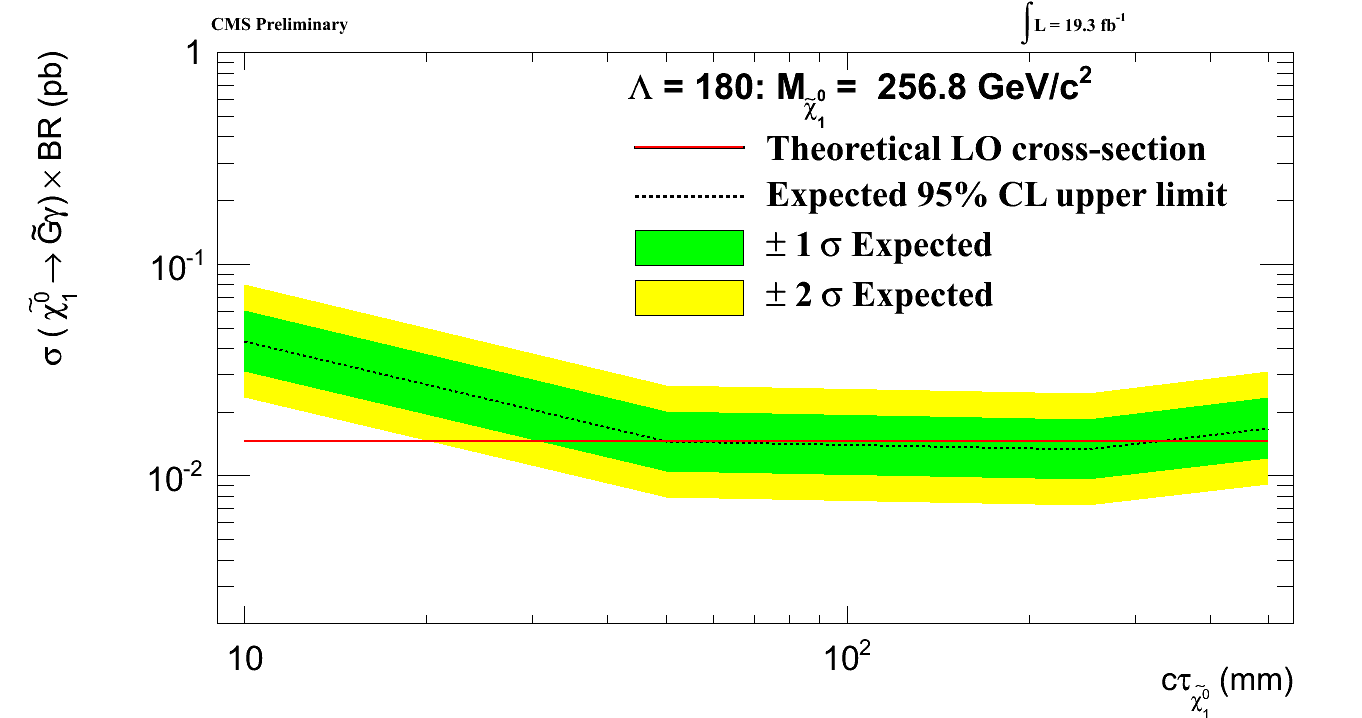
\includegraphics[width=\textwidth]{exclusionnoshapefinal.png}
\caption{Cut and count expected limit plot. The expected values as a function of the $\widetilde{\chi}^0_1$ proper decay length are shown by the dashed line. It indicates the expected median of results for the background-only hypothesis, while the green and yellow bands indicate the ranges that are expected to contain 68\% and 95\% of all observed excursions from the median, respectively. A cut on the $d_{XY} > 0.3$ cm optimizes the signal-over-background ratio. The expected limit plots are shown together with the theoretical cross section line.}
\label{fig:limitplotsnoshape}
\end{figure}



\begin{figure}[h]
\centering
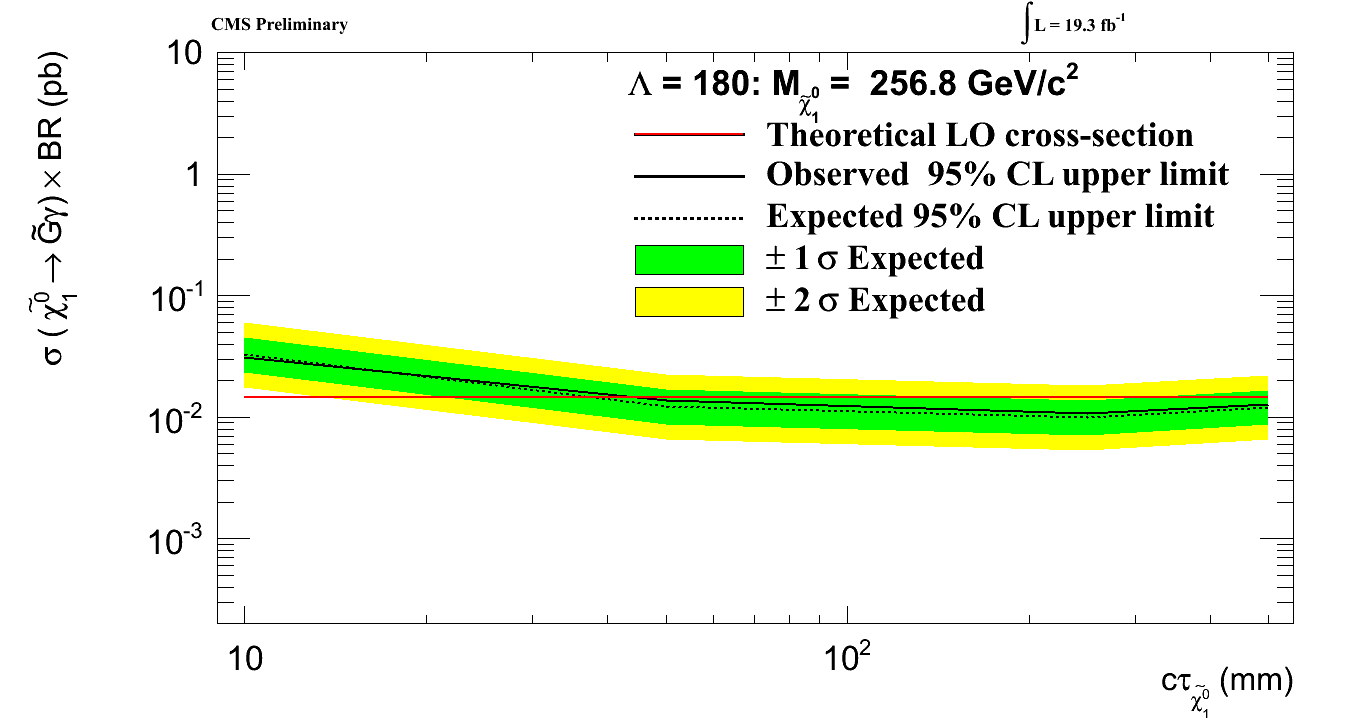
\includegraphics[width=\textwidth]{exclusionshapefinal.png}
\caption{Shape experiment for limit plots. The observed values as a function of the $\widetilde{\chi}^0_1$ proper decay length are shown by the solid line. The dashed line indicates the expected median of results for the background-only hypothesis, while the green and yellow bands indicate the ranges that are expected to contain 68\% and 95\% of all observed excursions from the median, respectively. This analysis not only looks at the absolute values of the $d_{XY}$ variable, but also at its shape in the signal, background and data samples.}
\label{fig:limitplotsshape}
\end{figure}




\begin{figure}[h]
\centering
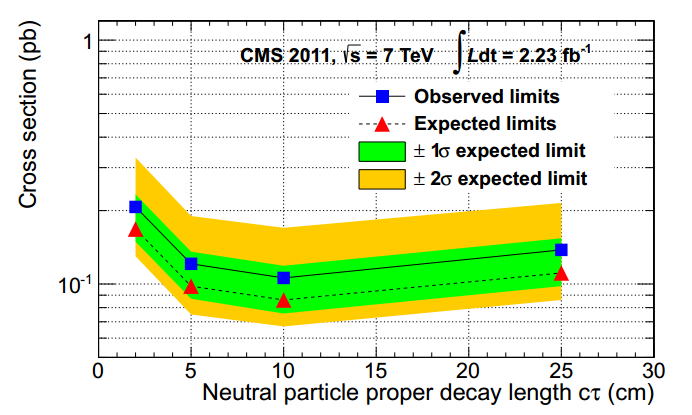
\includegraphics[9cm]{exclusionshapefinal7TeV.png}
\caption{Final result of the 7 TeV analysis. The observed values as a function of the $\widetilde{\chi}^0_1$ proper decay length are shown by the solid line. The dashed line indicates the expected median of results for the background-only hypothesis, while the green and yellow bands indicate the ranges that are expected to contain 68\% and 95\% of all observed excursions from the median, respectively.}
\label{fig:limitplotsshape7TeV}
\end{figure}


\chapter{Conclusion and Outlook}
\label{ch:conclusion}

The way to search for signals of new physics as predicted by theory models, such as supersymmetry, is not clear-cut. The reason for this is the multidimensional nature of these theories. Depending on the specific combination of model parameters, the predicted signal can look quite different. It is for this reason that experimental physicists often choose a certain signal model provided by their theoretical counterpart as the base for their search. Every model has its own specifics and characteristics. Even when we have chosen a model, there is no clear cut way to optimize our analysis. The search for SUSY is not easy as we have to search for everything/anything.\\
\\
In this analysis we performed a search for long-lived particles decaying into photons produced in association with jets. The photons then convert into $e^+e^-$-pairs where we reconstruct the impact parameter $d_{XY}$. This is our main discriminating variable to differentiate signal to background. We used LHC proton-proton collision data at a center-of-mass energy of 8 TeV corresponding to an integrated luminosity of 19.3 fb$^{-1}$. We interpret our analysis using a SUSY model with a GMSB scenario with a long-lived neutralino decaying to a photon and a gravitino. This model predicts that the gravitino, $\widetilde{G}$, is the Lightest SUSY Particle (LSP), while the $\widetilde{\chi}^0_1$ is the Next To Lightest SUSY Particle (NLSP). We estimated the dominant background with a data-driven approach. This is a method that was already used by the 7 TeV analysis where this thesis is based on. The method consists in selecting a control region in data rich in background events. Validation checks are made to ensure that our main search variable in the control region is invariant to the background in the signal region. If so, the background events in the control region can be used as background events in the signal region. After confirming that this data-driven method is suitable to model the background, the analysis was redone. A fit to the two-dimensional distribution in the main search variable yields no significant excess of events beyond the SM contributions, and upper limits at 95\% CL are obtained on the production cross section in the SPS8 model of GMSB supersymmetry.

\subsubsection{Outlook}
Due to time constraints, the analysis at hand could not be fully completed in the framework of this thesis. Some additional work is required to arrive at final results:

\begin{itemize}
\item Looking at a $\Lambda$ value of 160 TeV, corresponding to a higher cross section and giving us more statistics.
\item Proper computations of the systematic uncertainties can be done in the near future.
\item Checking the upper limits with a $c\tau > 50$ cm.
\end{itemize}


%%% DO NOT ADD \end{document}!
